\documentclass[11pt]{article}
\usepackage{LandP}
\usepackage{times}
\usepackage{latexsym}
\usepackage{graphicx}
\usepackage{amsmath}
\usepackage{multirow}
\usepackage{xspace}
\usepackage{url}

\usepackage[papersize={8.5cm, 5.5cm}, text={8.5cm, 5.5cm}]{geometry}

\begin{document}
\centering
%\scriptsize
\deriv{3}{
  \rm \hspace{1em}Disney\hspace{1em} & \rm \hspace{1em}acquired\hspace{1em} &\rm \hspace{1em}Pixar\hspace{1em} \\
\uline{1}&\uline{1}&\uline{1} \\
NP & S\bs NP /NP & NP \\ 

\includegraphics[scale=0.4]{tensor2}  &  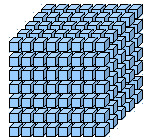
\includegraphics[trim=0em 0em 0em -0.2em,clip=true,scale=0.4]{tensor3}  & 
\includegraphics[scale=0.4]{tensor2} \\


& \fapply{2} \\
& \mc{2}{S\bs NP} \\
&  \mc{2}{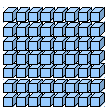
\includegraphics[scale=0.4]{tensor1}} \\
\bapply{3}\\
\mc{3}{S} \\
\mc{3}{
\includegraphics[scale=0.4]{tensor2}}
}
\setlength{\belowcaptionskip}{-10pt}
\end{document}